\documentclass[12pt]{article}   %  [titlepage]   \and
\usepackage{amsmath}
\usepackage[utf8]{inputenc}
\usepackage[T1]{fontenc}
\usepackage[danish]{babel}
\renewcommand{\rmdefault}{ptm}
\usepackage[pdftex]{graphicx}
\usepackage{multirow}
\newcommand{\nextitem}{\par\hspace*{\labelsep}\textbullet\hspace*{\labelsep}}

\title{Kalender \& booking til K. Translation}
\author{Omar Khalidan - [26-10-87]\\
     Morten Trolle Nielsen - [14-06-79]\\ \\
    Instruktor: Andreas Frisk\\ \\
Projekt i Systemudvikling 2014 (ProjDat2014)}

\begin{document}
\maketitle
\thispagestyle{empty}
\newpage
\tableofcontents
\newpage

\section{Abstract}
Dette er tredie delrapport i faget Systemudvikling. Vi vil fortsætte arbejdet med og præsentationen af den IT-løsning, som vi er ved at udvikle til kunden; tolkeservicen K. Translation. Vores udgangspunkt er første, anden og tredie delrapport, som vi har udviklet og udbygget. Vi har analyseret anvendelsesområdet, skrevet de vigtigste use cases og på den baggrund opstillet de funktionelle og ikke-funktionelle krav. Udfra dette arbejde har vi modelleret problemområdet. Vi har også lagt os fast på en softwarearkitektur, og brugergrænsefladen er blevet afprøvet ved hjælp af den første prototype og mock-ups.  \\
Vi vil afslutte denne fjerdie delrapport med to korte referater og efterfølgende analyse samt perspektivering af de to artikler, der er et krav til rapporten. Vi er selv førsteårs datalogistuderende ved Københavns Universitet, og det forventes, at læseren befinder sig på samme læringsniveau eller højere, idet der undervejs vil forekomme adskillige fagspecifikke termer. 

\newpage

\section{It-projektets formål og rammer}

Tolkeservicen K. Translation (KT) er et lille tolkebureau med speciale i arabiske 
sprog. Indehaveren af bureauet er Souzane, og hun er både leder og eneste
medarbejder i bureauet. Hendes kunder er offentlige myndigheder såsom politiet, anklagemyndigheden og diverse ministerier, samt private aktører såsom f.eks. advokatbureauer. Disse instanser kontakter K. Translation, når de har behov for en tolk til konkrete sager eller ved andet forefaldende tolkearbejde, og der laves en aftale. Det kan både være aftaler to eller tre uger ude i fremtiden, eller det kan ved mere presserende sager være aftaler med
kortere frist.\\
Ejeren af KT har ofte meget travlt både på arbejdet og i privatlivet, og på
den baggrund opstod ideen om en web-baseret kalender, der både kan dække hendes behov for en struktureret arbejdsdag og hendes kunders behov for hurtigt og nemt at kunne booke en aftale. Vi opsøgte Souzane, fordi vi mente, at denne opgave lå inden for rammerne af det mulige for et førsteårsprojekt. Det første møde fandt sted fredag den 21. marts, og vi blev enige om at begynde et samarbejde, der skal resultere i et færdigt kalender- og bookingsystem til KT og KT's kunder.
Kalendersystemet skal tilgås igennem en hjemmeside, hvor KT's kunder kan logge på systemet med brugernavn og password. \\
Når en af KT's kunder har logget på systemet, skal vedkommende præsenteres for en kalender. Kunden skal i kalenderen kunne se alle de tidspunkter, hvorpå det er muligt at booke en aftale med K. Translation. Når KT's kunde har besluttet sig for en dato og et tidspunkt, taster vedkommende dette ind i systemet. Derefter skal kunden oplyse typen på
arbejdet; om det er mundtligt eller skriftligt tolkearbejde, simultantolkning eller andet tolkearbejde. Aftalen gemmes så i databasen og vises herefter i kalenderen. KT's ejer har betonet vigtigheden af brugervenlighed, sådan at hendes samarbejdspartnere uden foregående undervisning 
hurtigt selv kan overskue kalenderen og booke en aftale. Slutteligt vil Souzane også have et system, hvor hun løbende kan tilføje nye samarbejdspartnere til den database, der gemmer på alle data. \\

\section{Anvendelsesområde}
Vi vil i dette afsnit påbegynde modelleringen af systemet. Vi begynder med at analysere den ene af de to centrale dele, nemlig anvendelsesområdet. Den anden del, problemområdet, vil vi modellere efter, at vi har gennemgået use cases og skrevet en kravspecifikation, så vores brugerforståelse og klarlæggelsen af systemfunktionaliteten kan ligge til grund for modelleringen af problemområdet. \\ 
Umiddelbart er anvendelsesområdet meget begrænset. Vi har fundet følgende klasser, der skal analyseres i anvendelsesområdet:

\begin{itemize}
\item K. Translation med indehaver (som samtidig er eneste medarbejder).
\item Systemadministrator kos K. Translation.
\item K. Translations kunder som politi, advokater, etc..
\item Eksternt, privat kalendersystem.
\end{itemize}

K. Translations indehaver Souzane, skal som den første medtages i anvendelsesområdet. Eftersom hun er eneste medarbejder i bureauet, kan hun potentielt set komme til at optræde i tre forskellige roller i anvendelsesområdet. For det første står hun som indehaver af K. Translation, så hun over for sine kunder bliver den ansvarlige for systemet, når det er færdigudviklet, implementeret og kører. For det andet bliver hun også en almindelig bruger af kalenderen, da hun kommer til at bruge den i sit daglige arbejde. Hun vil i et vist omfang selv komme til at ligge aftaler ind i kalenderen, og hun kan bruge den til at planlægge sin arbejdsdag. Endvidere skal hun selv oprette nye brugere til systemet, og derfor er overgangen til hendes tredie rolle som systemadministrator også flydende. Da hun ikke har andre ansatte, er det nødvendigt, at hun selv får en basal træning i systemadministration, så hun selv kan håndtere systemet på længere sigt, og derfor får hun også samtlige rettigheder, så hun kan tilgå hele systemet. Behovet for dette vil dog falde betragteligt, hvis vi placerer det endelige system hos et webhotel eller hos en anden udbyder af serverplads. \\
Vi vil i det videre arbejde antage, at Souzane er en "almindelig computerbruger", der er vant til at sende mails, bruge facebook og orientere sig på flere platforme. Men hun har også understreget nødvendigheden af, at den endelige it-løsning skal være let samt ukompliceret at gå til, så hun ikke skal bruge tid på systemets drift i hendes travle hverdag. \\
En anden klasse, der skal medtages i anvendelsesområdet, er KT's kunder og samarbejdspartnere. Kundegrundlaget er  
offentlige myndigheder som politi, ministerier, uddannelsessteder og hospitaler samt private aktører som advokater og andre samarbejdspartnere. Det kan f.eks være en politibetjent, der har brug for en arabisk tolk til en afhøring; en sekretær i dommervagten, der vil booke Souzane til en sag; eller et hospital, der skal operere en arabisk patient. \\
 Som det foregår nu, ringer kunderne til Souzane for at booke en tid, og det kan både være akutte henvendelser og henvendelser om tolkearbejde dage eller uger ude i fremtiden. Det er disse telefoniske henvendelser, vi gerne skal have kanaliseret igennem internettet og kalendersystemet i stedet for. Helt akutte sager, hvor Souzane bliver ringet op klokken to om natten, fordi der er brug for hende a.s.a.p., kan vi ikke gøre noget ved, men aftaler med længere frist kan med fordel placeres i kalenderen. \\
 KT's samarbejdspartnere har også brug for at få udført flere forskellige typer af tolkeopgaver. Der kan være mundtlige opgaver, hvor der skal simultantolkes. Og der kan være skriftlige opgaver (f.eks. et anklageskrift), som Souzane skal have oversat, når hun møder op på det pågældende tidspunkt. Derfor skal kunderne have mulighed for at vedhæfte dokumenter, når de booker en aftale i kalenderen. \\
Vi må forvente, at kundesegmentet har meget svingende it-kundsskaber, men at de i kraft af deres daglige arbejde er vant til at arbejde med diverse login- og kalendersystemer, der findes overalt i f.eks. den offentlige sektor. \\
Slutteligt har vi udvidet modellen med en ekstern kalenderklasse, der kan synkronisere Souzanes private kalender med vores kalendersystem og overføre hendes private
aftaler. Dette er et ønske fra Souzane, idet hun har en meget travl hverdag, hvor private aftaler godt kan ligge i vejen for arbejdsopgaver, og kunderne skal kunne se præcist, hvornår Souzane er tilrådighed. Det skal dog siges, at vi er meget usikre på denne funktion, og at vi potentielt må fortælle K. Translation, at dette ligger uden for vores formåen. I så fald må Souzane selv lægge sine egne aftaler ind i kalenderen. \\

\section{Use cases}
I dette afsnit vil vi beskrive systemets 4 vigtigste use cases. Udgangspunktet er anvendelsesområdet, hvor vi tager de forskellige aktører og simulerer et typisk handlingsforløb.  Resultatet skulle gerne være en øget brugerforståelse og en overordnet forståelse af systemfunktionaliteten. Dette arbejde kulminerer i næste afsnit med selve kravspecifikationen. \\
Vi begynder med at præsentere et højniveau-diagram over samtlige use cases, se figur \ref{fig:use}, og efterfølgende vil vi identificere de fire vigtigste use cases. 

\begin{figure}[!ht]
\begin{center}
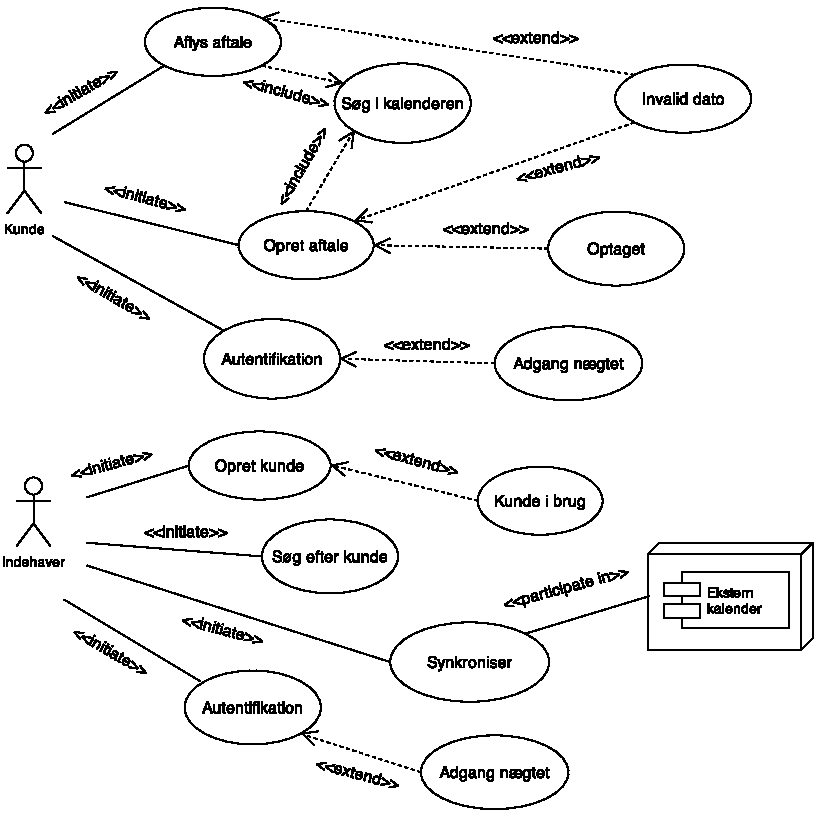
\includegraphics[width=12cm, height=12cm]{highlevel.pdf}
\caption{Højniveau use case diagram bestående af samtlige identificerede use cases.}
\label{fig:use}
\end{center}
\end{figure}

 
Aktørerne i højniveau use case diagrammet er alle hentede fra anvendelseområdet. Indehaveren af KT er i dette scenario også systemadministrator, idet hun selv vil
skulle udfylde denne rolle på længere sigt, og derfor er denne aktør ikke medtaget som en selvstændig klasse. Vi mener heller ikke, at det vil tilføje modellen mere værdi også at modellere systemadministratoren, da vedkommendes use cases i så fald vil være et subsæt af indehaverens.\\
Hvis to use cases indeholder det samme begrænsede handlingsforløb, har vi modelleret dette med et ``include'' forhold. F.eks. kan en potientel kunde søge i kalenderen,
både når vedkommende opretter en aftale, og når vedkommende aflyser en aftale. Dette er med til at nedsætte kompleksiteteten i use case modellen og fjerne redundans. Det samme gør sig gældende med ``extend'' forholdene, der modellerer undtagelser og fejltilstande som f.eks. systemets reaktion på ulovlige datoer eller mislykket login.\\
Vi har valgt de 4 vigtigste use cases ud og præsenterer dem her med sekvensdiagrammer. Første use case ``Opret kunde'' kan ses i tabel 1.\\

\begin{tabular}{l p{10cm}}
Use case navn & Opret kunde \\ \hline
Deltagere & \nextitem Initieret af KT's indehaver -
             Kommunikerer med kunde \\ \hline
Handlingsforløb &
	\nextitem Indehaveren af KT logger på systemet som administrator. 
	\nextitem Administratorinterfacet viser menuen.
	\nextitem Indehaveren navigerer til menupunktet, hvor man kan tilføje nye
		kunder.
		\nextitem Interfacet præsenterer en formular til indehaveren
	\nextitem KT's indehaver udfylder samtlige formularfelter med
		kundens stamdata og anden kontaktinformation. Derefter
		sender hun formularen.		
	\nextitem Administratorinterfacet tilføjer kunden til kundekartoteket
	og autogenererer en email, der sendes til den aktuelle kunde
		med besked om, at vedkommende nu kan logge på systemet for at
		booke en tid.
	\nextitem KT's indehaver logger af systemet. 
	\nextitem Interfacet lukkes.
	\\ \hline
	Indgangs betingelse &
		\nextitem KT's indehaver er logget på administratorinterfacet. 
		\nextitem Pågældende kunde er ikke oprettet i kundekartoteket. 
		\\ \hline
Exit betingelse & 
	\nextitem Pågældende kunde er nu tilføjet til
			kundekartoteket.
		\nextitem Der ligger en bekræftende email i den pågældende kundes
			indbakke.
		\nextitem KT's indehaver er logget af systemet.\\ \hline
\end{tabular}
\begin{center}
\textbf{Tabel 1} Opret kunde use case.
\end{center}
\vspace{0.5cm}

Denne use case beskriver, hvordan K. Translations indehaver opretter en ny kunde i kundedatabasen. I vores gennemgang vil vi fokusere på at identificere ``entity'', ``boundary'' og ``control'' objekterne i use casen, men vi vil dog i det efterfølgende bruge de danske betegnelser, som er henholdsvis entitet, grænseflade og kontrol. \\
De to aktører i use casen er KT's indehaver og en kunde. Indehaveren igangsætter use casen og er den aktive part, mens kunden kun medvirker passivt. Grænsefladeobjekterne i use casen er administratorinterfacet, hvor indehaveren
logger på systemet, og formularen, hvor hun indtaster kundens stamdata. Den bekræftende email er også en del af grænsefladen, selvom den ikke går til 
indehaveren men til kunden. Kundekartoteket er den ene entitet i use casen og kunde den anden. Her tænker vi ikke på kunden som aktør men som en entitet, der oprettes undervejs udfra de indtastede stamdata. Det er umiddelbart
lettere at identificere kontrollen i det medfølgende sekvensdiagram, så vi henviser til figur \ref{fig:opret}. Her fremgår det, at systemet har en administratorkontrol, der er ansvarlig for at oprette entiteten: Kunde og
grænsefladerne: Email samt Aftaleformular. Dette er måske snarere en for tidlig truffet design beslutning, men vi medtager den her, fordi kontrol objekter ofte udspringer af grænseflader, der tilgås af aktøren for at igangsætte 
handlingsforløbet.    

\begin{figure}[!ht]
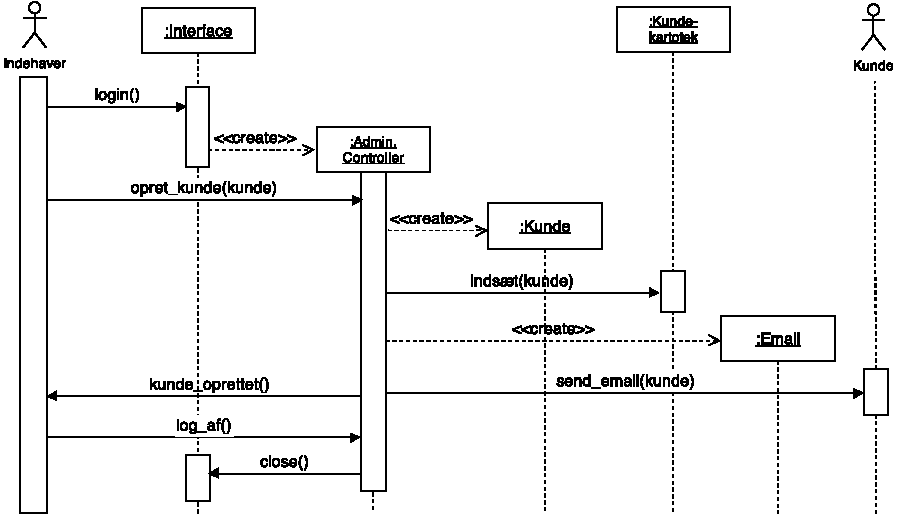
\includegraphics[width=14cm, height=10cm]{seqtwo.pdf}
\caption{Sekvensdiagram for Opret kunde use case.}
\label{fig:opret}
\end{figure}

Den anden use case, vi har valgt, hedder ``Opret aftale''. Se tabel 2.  Her 
logger en kunde på systemet for at booke en aftale med tolkeservicen, og
vedkommende skal både oplyse dato, klokkeslet og opgavetype. Igen er der to
aktører: kunden og KT's ejer. Men rollerne er byttede om i forhold til den
første use case. Nu er kunden den aktive part, og KT's ejer er den passive,
idet hun kun deltager i use casen for at modtage en email.\\


\begin{tabular}{l p{10cm}}
Use case navn & Opret aftale \\ \hline
Deltagere & \nextitem Initieret af KT's kunde
            - kommunikerer med Indehaveren af KT\\ \hline
Handlingsforløb &
	\nextitem KT's kunde navigerer til KT's hjemmeside, hvor kunden logger
	på med det personlige password.
	\nextitem Kalenderkontrollen henter kalenderen og viser den til
	kunden.
	\nextitem Kunden vælger at oprette en aftale.
	\nextitem Kalenderkontrollen henter en formular, som kunden skal
	udfylde.
	\nextitem Kunden indtaster datoen og klokkeslettet for den ønskede 
	aftale og bekræfter.
	\nextitem Kontrollen validerer dato samt klokkeslet og præsenterer
	kunden for en menu med forskellige aftaletyper.
	\nextitem Kunden vælger den ønskede aftaletype og bekræfter.
	\nextitem Kontrollen opretter aftalen i kalenderen og sender
	automatisk en email til både kunden og indehaveren af KT. 
	\nextitem Kunden logger af kalenderen.
	\\ \hline
	Indgangs betingelse &
		\nextitem KT's kunde er logget på kalenderen. 
		\nextitem Kalenderen indeholder ingen aftaler på det af kunden
		ønskede tidspunkt.
		\\ \hline
Exit betingelse & 
	\nextitem Der er oprettet en aftale i kalenderen på det ønskede
	tidspunkt. 
		\nextitem Der ligger en bekræftende email i den pågældende kundes
			indbakke.
		\nextitem Det ligger en email i KT's indehavers
			indbakke med dato og tidspunkt for aftalen. 
		\nextitem Kunden er logget af systemet.\\ \hline
		Kvalitets krav & Da det er muligt for kunden at søge i
		kalenderen, kan denne use case på et vilkårligt tidspunkt
		inkludere use casen  ``Søg i kalender''. Hvis dette sker, kan
		kunden søge i kalenderen, enten ved at bladre frem èn dag eller uge
		ad gangen eller ved at søge på en dato længere ude i
		fremtiden.\\ \hline
\end{tabular}
\begin{center}
\textbf{Tabel 2} ``Opret aftale'' use case.
\end{center}
\vspace{0.5cm}


Grænsefladeobjekterne er KT's hjemmeside, som use casen indledes fra, og
formularerne, der udfyldes af kunden undervejs. Den bekræftende email er
ligeledes en del af grænsefladen. Kalenderen og aftalen er entiteter, og som
det fremgår af det medfølgende sekvensdiagram, så udgøres kontrolobjektet af en
``kalender controller''. Se figur \ref{fig:aft}. 
Igen består første kolonne af den initierende aktør, anden kolonne er
grænsefladen, som aktøren bruger til at igangsætte use casen, og tredie
kolonne indeholder kontrol objektet, som undervejs når at oprette to
grænsefladeobjekter mere samt endnu en entitet.

\begin{figure}[!ht]
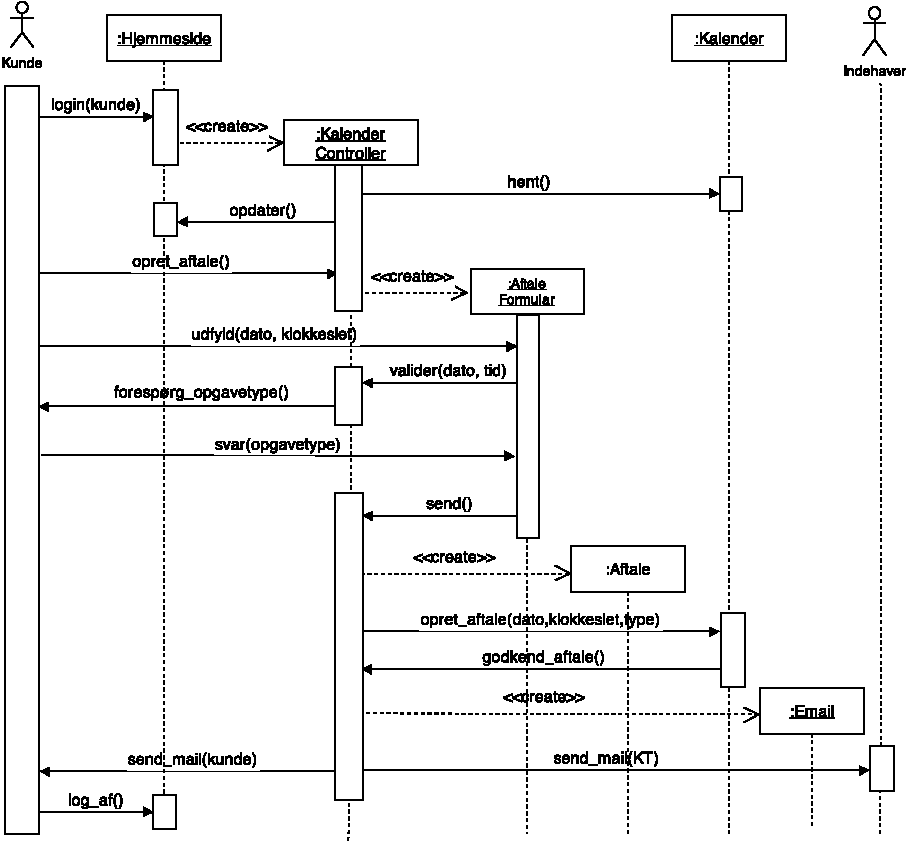
\includegraphics[width=14cm, height=11cm]{seq.pdf}
\caption{Sekvensdiagram for ``Opret aftale'' use case.}
\label{fig:aft}
\end{figure}

Efter at have vist to almindelige use cases, har vi til sidst valgt, at fokusere på de extraordinære forhold, der gør sig gældende ved ``extend'' use cases. Derfor viser vi to små use cases: ``Optaget'' og ``Ulovlig dato'', men vi gennemgår kun selve undtagelserne, eftersom konteksten for
disse use cases er ``Opret aftale'' use casen fra tabel
2 og sekvensdiagrammet i figur \ref{fig:aft}. Handlingsforløbene før og efter, undtagelserne træder i
kraft, vil være præcise gentagelser af ``Opret aftale'' use casen; man skal
altså forestille sig denne use case på et givent tidspunkt i forløbet
blive udvidet med en af de følgende to use cases. Se tabel 3 og 4.\\ 



\begin{tabular}{l p{10cm}}
Use case navn & Optaget \\ \hline
Deltagere & \nextitem Kommunikerer med KT's kunde. 
            \\ \hline
Handlingsforløb &
	\nextitem Kunden oplyser typen på opgaven og bekræfter. 
	\nextitem Kalenderkontrollen prøver at oprette en aftale i kalenderen
	på det givne tidspunkt, men bliver nægtet adgang, fordi der allerede
	ligger en aftale på dette tidspunkt. Kontrollen beder kunden om at
	finde en ny tid.
	\nextitem Kunden indtaster et nyt tidspunkt i formularen og bekræfter. 
	\nextitem Formularen validerer tidspunktet.
	\\ \hline
	Indgangs betingelse &
		\nextitem Denne use case udvider ``Opret aftale'' use casen.
		Den initieres, når kontrollen prøver at indsætte en aftale i
		kalenderen på et tidspunkt, hvor der i forvejen eksisterer en
		aftale. 
		\\ \hline
Exit betingelse & Kunden har oprettet en gyldig aftale i kalenderen.
	\\ \hline
\end{tabular}
\begin{center}
\textbf{Tabel 3} ``Extend'' use case: ``Optaget''.       
\end{center}
\vspace{0.5cm}


\begin{tabular}{l p{10cm}}
Use case navn & Ulovlig dato \\ \hline
Deltagere & \nextitem Kommunikerer med KT's kunde.
            \\ \hline
Handlingsforløb &
	\nextitem Kunden oplyser kontrollen om, at vedkommende vil oprette en
	aftale.
	\nextitem Kontrollen opretter en formular til aftalen.
	\nextitem Kunden indtaster dato og klokkeslet for aftalen og
	bekræfter.
	\nextitem Formularen prøver at validere tidspunktet, men den fejler.
	Kontrollen beder kunden indtaste et nyt tidspunkt.
	\nextitem Kunden indtaster dato og klokkeslet for den nye aftale og
	bekræfter.
	\nextitem Formularen prøver at validere tidspunktet og godkender.
	Kontrollen spørger kunden om opgavetypen.
	\nextitem Kunden oplyser opgavetypen og bekræfter.
	\\ \hline
	Indgangs betingelse &
		\nextitem Denne use case udvider ``Opret aftale'' samt ``Aflys
		aftale'' use cases. Den initieres, når formularen ikke kan
		validere tidspunktet for kundens aftale, fordi kunden har
		indtastet et ikke eksisterende tidspunkt.  
		\\ \hline
Exit betingelse & Der ligger en gyldig aftale i kalenderen på en lovlig dato.
	\\ \hline
\end{tabular}
\begin{center}
\textbf{Tabel 4} ``Extend'' use case: ``Ulovlig dato''.       
\end{center}
\vspace{0.5cm}

Grænseflade-, kontrol- og entitetobjekterne i de to ``extend'' use cases vil
være magen til objekterne i de oprindelige use cases, der udvides med disse
undtagelser, som det også fremgår af de medfølgende sekvensdiagrammer. Se figur
\ref{fig:extseq} for begge sekvensdiagrammer. \\

\begin{figure}[!ht]
\begin{center}
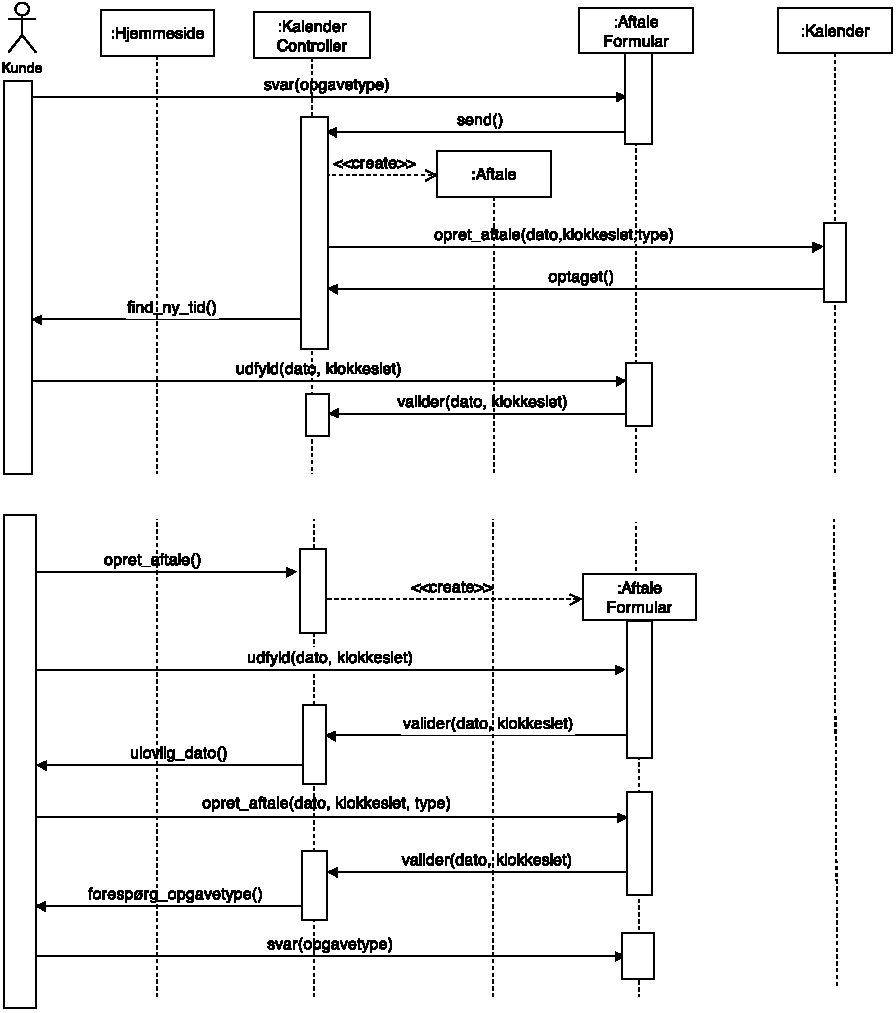
\includegraphics[width=13cm, height=15cm]{ext.pdf}
\caption{Sekvensdiagram for ``Optaget'' samt  ``Ulovlig dato''.}
\label{fig:extseq}
\end{center}
\end{figure}

Vores arbejde med disse use cases og sekvensdiagrammer har betydet, at vi har oplevet systemet fra brugerens synsvinkel, og at vi således har lagt fundamentet for kravspecifikationen. Derudover har vi med ``extend'' use cases set, hvorhenne i systemet undtagelser og exceptionel opførsel kan blive et problem, der skal håndteres. Vi har valgt at identificere grænseflade-, kontrol- og entitetobjekter allerede på nuværende tidspunkt, så dette arbejde bl.a. kan ligge til grund for et senere afsnit om softwarearkitektur og designmønster. 


\section{Projektaftale}
Før vi fortsætter med modelleringen af problemområdet, vil vi beskrive præcist, hvilke krav og forventninger kunden K. Translation har til vores endelige løsning. Vi har delt den følgende kravspecifikation op i to dele: funktionelle krav, som dækker samspillet mellem anvendelsesområdet og
kalender- samt bookingsystemet uden implementeringsspecifikke detaljer. Og non-funktionelle krav, der dækker over ikke direkte funktionelle aspekter som bl.a. brugervenlighed og pålidelighed. Idet kravspecifikationen senere ligger
til grund for afprøvningen af systemet, er det vigtigt, at den er ``komplet, konsistent, entydig og korrekt.''\cite{oose}[p.~122] \\

\subsection{Funktionelle krav}
På det første kundemøde beskrev indehaveren af K. Translation, hvilke forventninger og ønsker hun havde til det færdige produkt: et integreret kalender- og bookingsystem. Vores arbejde med anvendelsesområdet og use cases betyder, at vi nu kan opstille de funktionelle krav, der udgører rammerne, indenfor hvilke vi udvikler systemet. De funktionelle krav kan ses i den følgende liste.\\

\rule{120mm}{1mm}
\begin{itemize}
\item K. Translation ønsker en it-løsning, som af bureauets kunder kan tilgås over internettet via en hjemmeside.
\item På hjemmesiden skal KT's kunder præsenteres for en login menu, hvor de logger på systemet med et brugernavn og et password.
\item It-løsningen skal indeholde en kalender med ledige og optagede tidspunkter.
\item Der skal være et tilhørende bookingsystem, så kunderne kan lave en aftale med KT.  
\item Det skal være muligt for kunderne at søge i kalenderen efter ledige tidspunkter. Søgekriterierne er dato og klokkeslet. 
\item KT's kunde skal vælge typen på arbejdet inden for et antal forudbestemte kategorier.
\item Der skal sendes en bekræftende email tilbage til kunden, efter at vedkommende har booket en tid i kalenderen. 
\item KT modtager ligeledes en email med dato, klokkeslet, kunde og opgavetype.
\item Det skal være mulig for kunderne at aflyse en aftale.
\item Det skal være muligt for K. Translation løbende at tilføje flere kunder eller samarbejdspartnere til databasen. 
\item KT's indehaver vil gerne kunne overføre sine private aftaler fra en ekstern kalender til vores kalendersystem. Hun forestiller sig en form for synkronisering, men vi har fra start gjort hende det klart, at dette måske for os er en for kompliceret opgave. 
\end{itemize}
\rule{120mm}{1mm}
\vspace{0.5cm}

Vi har i samarbejde med Souzane udviklet den ovenstående liste af funktionelle krav, da KT fra start havde et godt billede af, hvilke funktioner og egenskaber det færdige produkt skulle indeholde. Vi synes, at de funktionelle krav på en god og dækkende måde beskriver de ønsker, som K. Translation har til det færdige program. Det skulle være muligt at teste, om vores løsning lever op til alle ovenstående krav, når systemet senere skal valideres på baggrund af kravspecifikationen.  \\ 


\subsection{Non-funktionelle krav}
Indehaveren af K. Translation kom også med nogle forventninger og ønsker, som ikke umiddelbart hører under systemets funktionelle egenskaber. Det er bl.a. forventninger om brugervenlighed, pålidelighed og andre svært verificerbare
egenskaber. Disse ønsker har vi samlet her i afsnittet med de non-funktionelle krav sammen med mere  implementeringsspecifikke detaljer. Den følgende liste
indeholder de non-funktionelle krav til systemet.\\

\rule{120mm}{1mm}
\begin{itemize}
\item Hjemmesiden skal indeholde K. Translations kontaktinformationer.
\item Designet skal være enkelt	og intuitivt, så personer uden store it-forudsætninger kan navigere på siden og booke en tid.
\item Souzane ønsker et design med lyse pastelfarver iblandet sort. 
\item Alle brugere skal kunne tilgå systemet med en almindelig web browser som Internet Explorer, Firefox eller Google Chrome.
\item KT ønsker et system af farvekoder, så kunderne hurtigt og nemt i kalenderen kan skelne de forskellige aftale- samt opgavetyper fra hinanden.
\item K. Translation ønsker den letteste og billigste implementering og hosting af systemet.
\item Indehaveren vil have et system, der ikke kræver løbende
	vedligeholdelse, men som bare ``kører og passer sig selv''.   
\item Der ønskes præcis og let forståelig dokumentation af systemet. 
\item Kalendersystemet og backend databasen må ikke tabe data eller aftaler, da dette betyder tabt indkomst for KT.
\end{itemize}
\rule{120mm}{1mm}
\vspace{0.5cm}

Som det fremgår, vil flere af de nonfunktionelle krav være svært verificerbare. Det er meget svært at fastslå med nogen som helst sikkerhed, hvornår en bruger opfatter en hjemmeside som enkel, intuitiv eller let at overskue. Man kan stille
parametre op, fastsætte gennemgående regler for designet og bruge afprøvede metoder, men der kan alligevel ikke gives nogen garantier. Derfor vil vi også i en senere rapport bruge tænke-højt-forsøg for at få en ide om, hvor godt
eller dårligt vores design er i forhold til disse egenskaber. \\
 Andre af de non-funktionelle krav udspringer af manglen på it-kompetancer internt i bureauet og af fraværet af en systemadministrator. Dette betyder højest sandsynligt, at vi 
placerer det færdige system hos en udbyder af serverplads, da KT i så fald kommer til at stå for et minimum af systemvedligehold. Det vil også være den billigste
løsning, da anskaffelsen af en server, strøm og evt. køling vil resultere i en betragtelig merudgift. \\
Da belastningen af systemet ikke forventes at blive særlig høj, har KT. ingen performancemæssige krav til vores løsning. Der er ingen tidskritiske brugerfunktioner, og risikoen for samtidig brug af kalenderen må forventes at være minimal. Man kunne godt forestille sig to kunder, der vil booke den samme 
tid i kalenderen med race condition til følge, men backend
databasens transactionindstillinger burde kunne håndtere dette
tilfredsstillende. Pålidelighed er på den anden side et vigtigt punkt, da K. Translation ikke kan acceptere, at aftaler tabes eller forsvinder. \\ 


\section{Problemområde}
Vi har nu gennemgået anvendelsesområdet, identificeret de vigtigste use cases og skrevet en kravspecifikation. Derfor kan vi nu på baggrund af dette arbejde gå igang med at modellere problemområdet. Vi præsenterer for overskuelighedens skyld først et UML-diagram over området. Se figur \ref{fig:problem}. Dernæst kommer der en kort opsummerende liste med klasserne efterfulgt af et længere forklarende afsnit.  

\begin{figure}[!ht]
\begin{center}
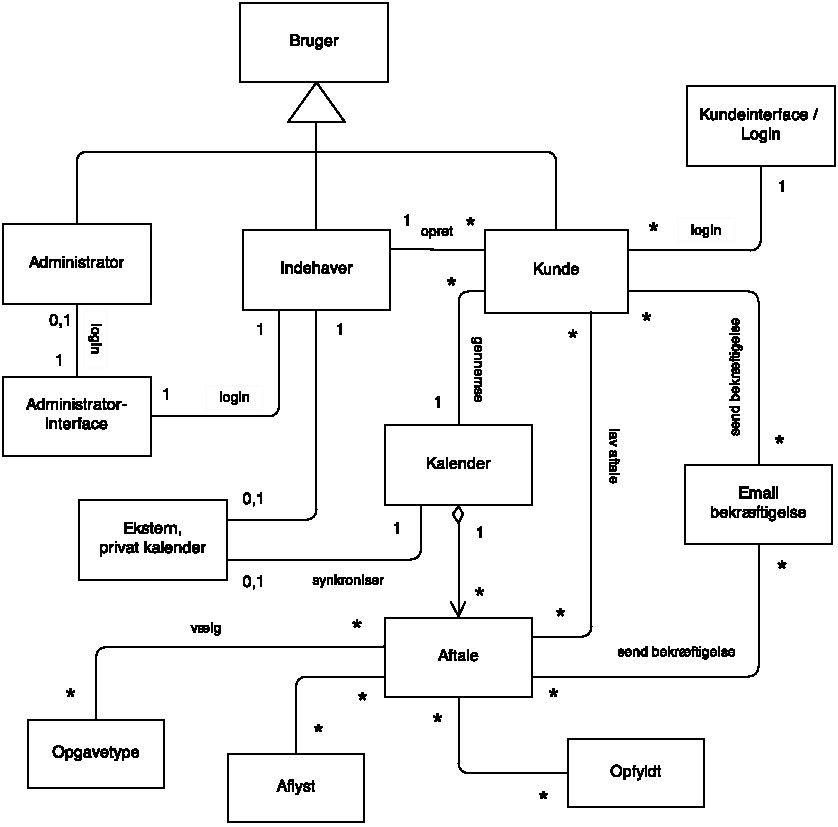
\includegraphics[width=12cm, height=12cm]{problemomr.pdf}
\caption{UML-diagram over problemområdet}
\label{fig:problem}
\end{center}
\end{figure}

Her følger en liste af de klasser, vi har identificeret i problemområdet:

\begin{itemize}
\item Bruger: Kunde, administrator, indehaver. Går igen fra
	anvendelsesområdet.
\item Et kundekartotek, hvor KT's indehaver løbende kan tilføje kunder.
\item Kalenderen, som kunderne kan bruge, når de skal finde en ledig tid, og som KT's indehaver kan bruge i sit daglige, travle arbejde.
\item Aftale. Kunderne booker en aftale i kalenderen.
\item Da KT har både mundtlige, skriftlige og andre opgaver, skal kunden	oplyse typen på arbejdet.
\item Kunden får en bekræftende email tilsendt med det aftalte tidspunkt.
\item KT's indehaver får ligeledes en påmindelse tilsendt pr. email, når der er oprettet en aftale i kalenderen. 
\item KT's indehaver har et ønske om at kunne synkronisere hendes eksterne, private kalender med vores it-løsning.
\end{itemize}

Det første, vi har modelleret, er brugerne fra anvendelsesområdet, idet disse skal have adgang til klasserne i problemområdet. Souzane skal kunne oprette nye kunder i kundekartoteket, og eksisterende kunder står opførte i dette kartotek. Derfor har vi modelleret en kartotekklasse imellem Souzanne og klassen Kunde. Endvidere skal Souzane kunne tilgå kalenderen for at tjekke aftalerne og evt. selv lægge nye private eller indtelefonerede aftaler ind. \\
Klassen Kunde vil efter login have adgang til klassen Kalender, hvor de har mulighed for at søge efter ledige tidspunkter til en aftale. Dette fører modelleringen videre til Aftaleklassen, og eftersom der vil være en naturlig sammenhæng mellem kalender og aftale, er de sammenkoblet ved aggregering. Da en aftale både kan være aflyst og opfyldt, vil klassen Aftale indeholde en attribut, der markerer denne forskel. Når kunden har booket en aftale vil vedkommende automatisk modtage en bekræftende email med dato og tidspunkt. Dette ses til højre i UML-diagrammet, hvor emailen autogenereres og sendes tilbage til kunden. Souzane vil ligeledes modtage en påmindende email, hvilket ses til venstre i diagrammet. \\
Det sidste, vi vil berøre i problemområdet, er det usikre punkt om samspillet mellem en ekstern kalender og vores eget kodede kalendersystem. Vi har modelleret en Ekstern Kalenderklasse til Souzanes egen private iCloud kalender, som hun gerne vil synkronisere med vores it-løsning for at overføre hendes private aftaler, så alt er samlet i èn
kalender. Men da denne opgave måske er for kompliceret for os, har vi forklaret Souzane, at private aftaler måske skal indtastes manuelt i kalenderen. \\
Hermed slutter vi gennemgangen af problemområdet. Den ovenstående modellering vil ligge til grund for det videre design og endelige system. 

\section{Softwarearkitektur}

Vi vil nu prøve at samle trådene fra de forrige afsnit og lægge os fast på en softwarearkitektur. Vi har overvejet flere forskellige arkitekturer og vil argumentere for vores valg og fravalg. Først overvejede vi en multilagdelt arkitektur i form af 3-tier arkitekturen. Her kunne vi i
datalaget gemme de oprettede brugere og bookede aftaler i en database. Forretningslogikken kunne placeres i mellemlaget og kodes med PHP. Brugerinterfacet ville ligge i præsentationslaget og tilgås gennem brugerens
browser. Vi fravalgte dog denne løsning af flere grunde. Vi fandt det ikke strengt nødvendigt med tre lag, da det tredie lag ikke ville betyde nævneværdige forbedringer i forhold til en almindelig client-server model. Derudover kunne vi også uforvarent komme til at introducere flere sikkerhedsbrister, hvis vi havde kodet mellemlaget i PHP, da dette kræver, at 
man er ekstrem opmærksom på validering af brugerinput. Da vores kalendersystem ikke kræver andet for at fungere end en bruger med en browser, der kan logge på KT's server, besluttede vi derfor, at holde arkitekturen så overskuelig som mulig ved at bruge client-server modellen. \\
Dernæst valgte vi at implementere systemet med det Model-View-Controller (MVC) baserede webframework Django. Se figur \ref{fig:mvc}.\\

\begin{figure}[!ht]
	\centering
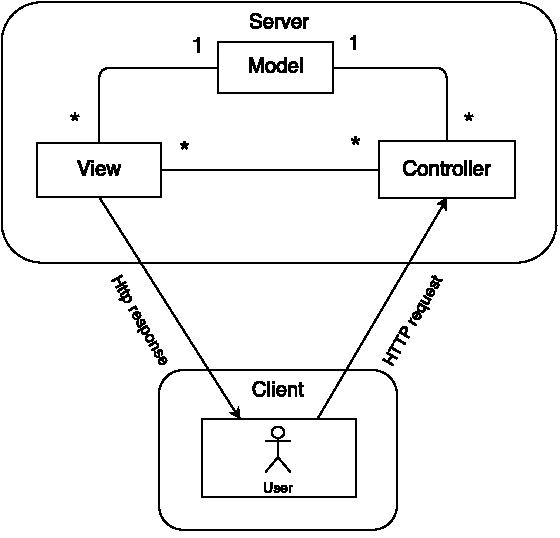
\includegraphics[width=6.5cm, height=5.5cm]{mvc.pdf}
\caption{Model-View-Controller arkitektur superimposeret på client-server.}
\label{fig:mvc}
\end{figure}

Django kommer med et enkelt og praktisk administratorinterface, der kan blive
særdeles nyttigt for os under systemudviklingen og for indehaveren af KT på længere sigt. Desuden får vi mulighed for at benytte Django's mange indbyggede applikationer. Vi kommer til at bruge moduler, der understøtter implementering af html formularer, og som også er i stand til at validere brugerinput i disse, og moduler for brugeroprettelse og autentifikation. Det betyder for os, at der er
færre muligheder for at introducere fejl og sikkerhedsmangler til systemet. En af Djangos helt store styrker, som udspringer af MVC arkitekturen, er den løse kobling og strenge adskillelse mellem de forskellige dele af modellen. Det betyder, at vi let kan ændre, slette eller tilføje i eksisterende dele uden at bekymre os om afhængigheder mellem delene. \\
Valget af Django skal også ses i forhold til vores arbejde med use cases og sekvensdiagrammer. Vi fokuserede på at identificere entiteterne(entity), grænsefladerne(boundary) samt kontrollerne(control), og disse objekter kan nu kortlægges til Model, View og Controller. Derfor har vi allerede nu afgrænset objekternes opførsel, og vi kan hurtigt sætte dem ind i en MVC kontekst. \\
Eftersom views i Django terminologi består af templates, og controllers består af viewfunktioner, er det måske mere rigtigt at kalde Django for en Model-View-Templates
(MTV) arkitektur, men vi bibeholder den normale konvention og skriver MVC. Vores model kommer til at bestå af de aftaler, som KT's kunder booker ind i kalenderen. D.v.s at domænerne i den bagvedliggende database, som modellen kortlægges til og 
fra, udgøres af datoen og klokkeslettet for aftalen, opgavetypen samt navnet på kunden. Django's templates står som sagt for præsentationen, og vi påtænker at bruge en basisskabelon til hjemmesiden, der kan udvides med
tilpassede templates, når logikken kræver det. Selve forretningslogikken bliver implementeret i Django's viewfunktioner. (Controller i MVC). Det er bindeleddet
mellem modellen og præsentationen, og det er her kernefunktionaliteten kommer til at sidde. Eftersom Django i virkeligheden er en samling Python biblioteker, vil vi kode 
systemet i programmeringssproget Python. Det er også et godt valg, fordi det ene medlem i vores tomandsgruppe har erfaring med Python, og det andet medlem ikke har. Python kan læres relativt hurtigt, så det ene medlem får muligheden for at
lære det undervejs i projektet, mens det andet medlem kan lære det fra sig evt. gennem pair-programming. \\ 

\section{Brugergrænseflade}
\subsection{Brugergrænseflade og flowcharts}
Vi er nu nået så langt i projektudviklingen, at vi kan begynde at arbejde med designet og brugergrænsefladen. Vi præsenterer her den første prototype af systemet ved hjælp af mock-ups og screen-shots af det påtænkte design. Derudover tegner vi de vigtigste flowcharts, så vi kan få et overblik over dynamikken i systemet. Vi vil få en person, der ikke er tilknyttet projektet, til at gennemgå vores prototype mock-up. Det mest ideelle ville dog have været, at få en virkelig bruger af det endelige kalendersystem, til at evaluere prototypen, men det har ikke været muligt på nuværende tidspunkt. Vi er dog af Souzane blevet stillet i udsigt, at vi sagtens kan få flere endelige brugere af kalenderen til at teste den færdige version, når dette engang bliver aktuelt, og det er selvfølgelig en unik mulighed, vi har tænkt at benytte os af. \\
Det første flowchart viser dynamikken i systemet fra en bruger logger på til vedkommende logger af. Se figur \ref{fig:flow1}.\\

\begin{figure}[!ht]
\begin{center}
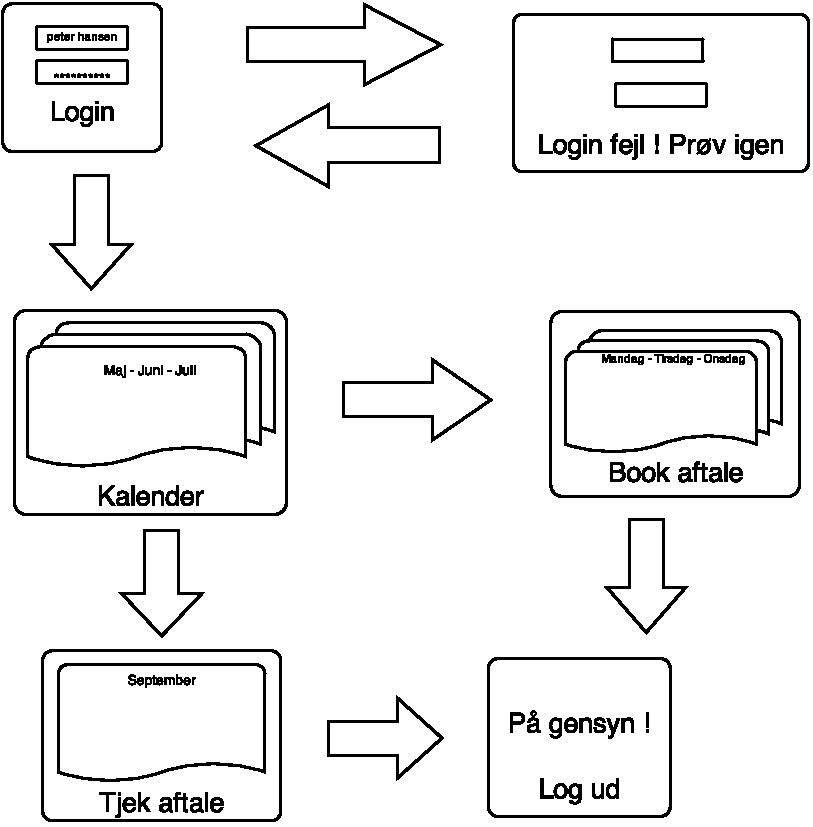
\includegraphics[width=8cm, height=8cm]{flow1.pdf}
\caption{Flowchart over kalendersystemet}
\label{fig:flow1}
\end{center}
\end{figure}

Brugeren vil efter succesfuldt login blive dirigeret videre til en side, der viser den aktuelle måned. Det skal være muligt for brugeren at trykke sig fremad månedsvis, så vedkommende kan indsætte en aftale i kalenderen uger eller måneder ude i fremtiden, men det skal ikke være muligt at bladre tilbage i kalenderen, eftersom dette ikke vil bibringe kalenderen nogen merværdi. Brugeren kan nu vælge mellem to veje: enten at tjekke kalenderen igennem uden at oprette eller aflyse nogen aftaler, eller vedkommende kan vælge at redigere i kalenderen. Vi har tegnet et nyt flowchart, der viser forløbet, hvis brugeren vælger at redigere i kalenderen. Se venstre side af figur \ref{fig:flow2}. Dette udvikler det første overordnede flowchart, og vi har bl.a. brugt sekvensdiagrammerne samt de relevante use cases fra afsnit 4 til at udvikle brugergrænsefladen, så der er overensstemmelse mellem de forskellige designfaser. \\


\begin{table}[ht]
\centering
\begin{tabular}{l | r}
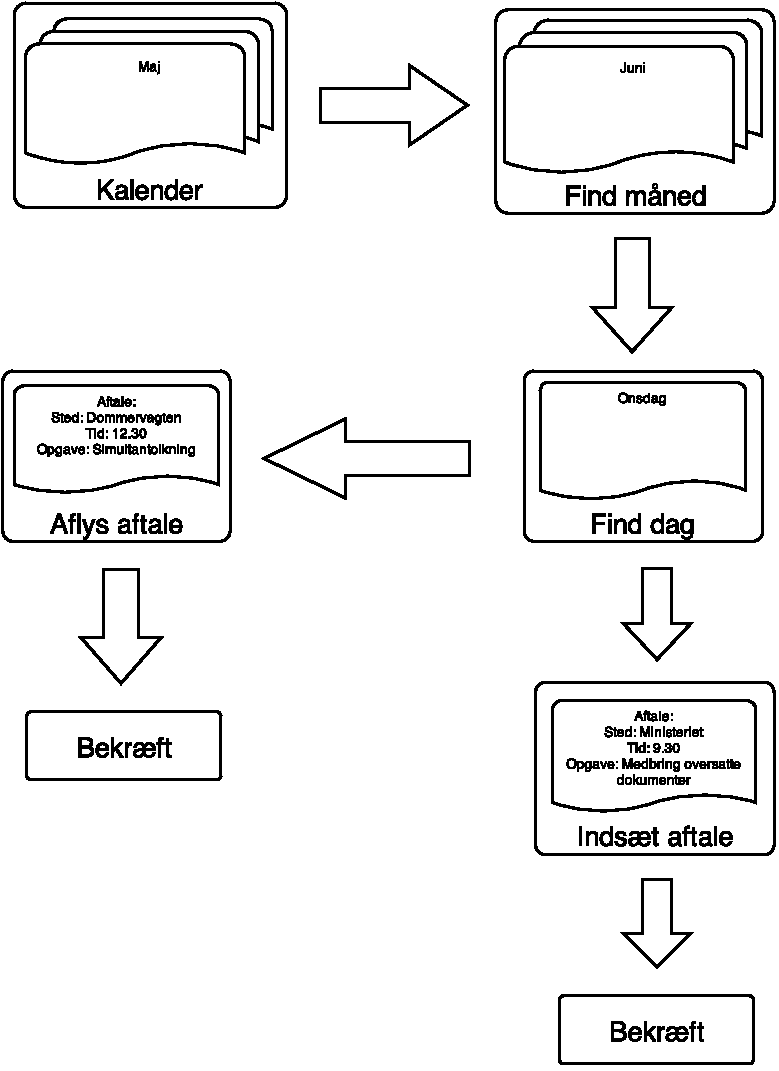
\includegraphics[height=7cm,width=7cm]{flow2.pdf}
\label{fig:flow2}&
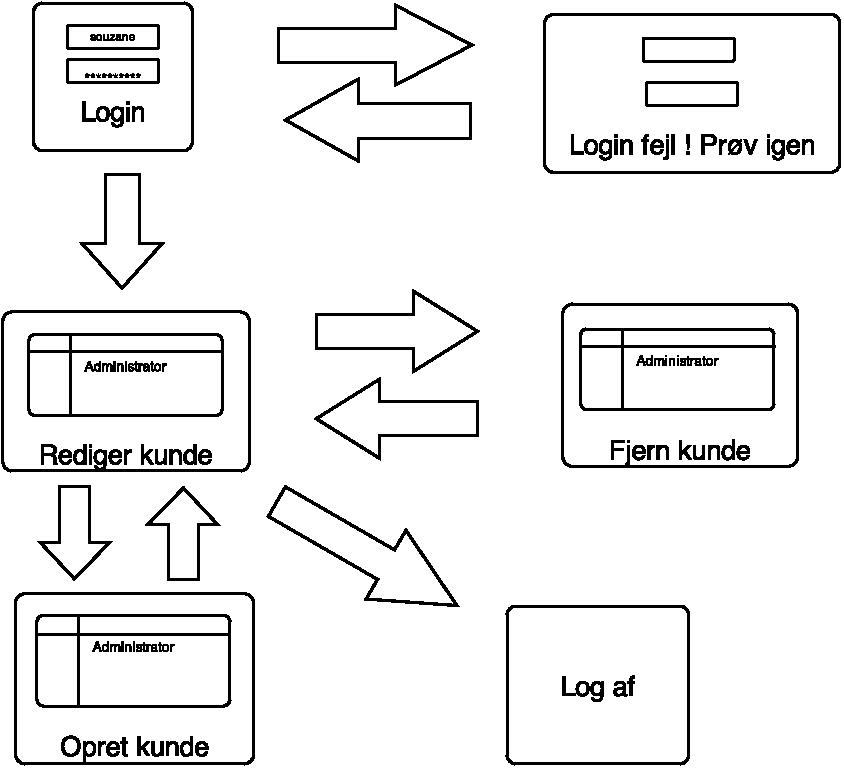
\includegraphics[height=7cm, width=7cm]{flow3.pdf}
\\
\end{tabular}
\label{tab:gt}
\end{table}
\begin{centering} \textbf{Figur \ref{fig:flow2} og 8.2 :} To flow-charts. Det venstre viser navigation i kalenderen samt oprettelse og aflysning af aftale. Det højre viser oprettelsen af en kunde. 
\end{centering}

\vspace{0.5cm}

Flowchartet viser de to veje, man kan følge, hvis man enten skal aflyse eller oprette en aftale. Højre side af figur \ref{fig:flow2} viser forløbet, hvis Souzane enten skal oprette eller fjerne en kunde i systemet. Vi vil ikke gøre mere ud af disse flowcharts, men i stedet for gå videre til den prototype af kalenderen, vi har designet i form af mock-ups. \\

\subsection{Prototype, mock-ups og tænke-højt-forsøg}
Vi har nu lagt os fast på et design af kalenderen, og vil gerne have det testet af en bruger, inden vi begynder at kortlægge modellen til kode. Derfor har vi lavet en mock-up model af kalendersystemet bestående af 5 tegninger, der, når de vises i den rigtige rækkefølge, kan gøre det ud for et normalt handlingsforløb, som det vi så i use casen "Opret aftale" fra afsnit 4, og som det også fremgik af forrige flowcharts. \\
Alle fem mock-up tegninger kan ses i korrekt rækkefølge i bilag 1, men de er grundet pladshensyn ikke taget med her. Vi har som sagt ikke testet mock-up'en på en rigtig end-user, men har fået vores kammerater, der alle selv er igang med lignende projektforløb, til at teste modellen ved et tænke-højt-forsøg. Det betyder, at vi får svært ved at sætte kalenderen ind i en rigtig kontekst, da vi ikke kan simulere en travl arbejdsdag med telefoner, der ringer, og møder, der skal nås. Til gengæld håber vi på, at fordi vores kammerater selv er igang med lignende projekter, så har de en nysgerrig og professionel tilgang til opgaven. \\
Testen forløb på den måde, at en testperson blev stillet en opgave, der lød: Book en aftale i kalenderen. Derefter blev personen præsenteret for den første tegning med en login menu, og når vedkommende havde udfyldt denne korrekt, så fik personen næste tegning fremlagt. Dette fortsatte indtil, at der var oprettet en aftale i kalenderen, og testpersonen havde modtaget en bekræftigelse på aftalen. Mens vi præsenterede personen for tegningerne, overvågede Omar og jeg forløbet, og vi lagde mærke til, hvor testpersonen havde let ved at forstå designet, og hvor der var misforståelser og forvirring. Vi måtte ikke kommunikere med testpersonen undervejs, medmindre vedkommende sad fuldstændig fast, men udelukkende lytte til hvilke overvejelser, testpersonen gjorde sig undervejs. Bagefter evaluerede vi forsøget med testpersonen. Her har vi samlet nogle af de hyppigste bemærkninger:

\begin{itemize}
\item Enkelt og simpelt design.
\item De var en, der mente, at det måske var for simpelt. Vedkommende kunne godt tænke sig nogle flere funktioner som f.eks. en hjælpe- / supportfunktion.
\item Der var lidt forvirring om, hvordan man kom fra månedskalenderen til dags dato-visningen. Nogle troede, at pilen til at navigere frem i kalenderen ville føre dem til den valgte dag. 
\item Ellers blev månedskalenderen opfattet som overskuelig og nem at gå til. 
\item Der var nogen forvirring omkring, hvordan man lægger en aftale ind under dags dato.
\item Der var flere, der begyndte at indsætte aftalen allerede på mock-up tegning 3. 
\item Det var ikke helt klart for testpersonerne, hvordan de skulle booke en aftale, hvor tidsintervallet måske var 4 timer. De forsøgte enten at skrive aftalen ind hver halve time, eller at markere et større tidsinterval med musen.
\item Der var nogle, der mente, at det krævede for mange videre-klik af booke en aftale, og at der var for mange forskellige skærmbilleder undervejs i forløbet. De syntes, at vi skulle overveje at forenkle designet. Folk, der logger ind på kalenderen, ved som regel præcist, hvornår de vil booke en aftale, og for dem vil det være et irritationsmoment at skulle igennem flere irrelevante skærmbilleder. 
\item Der var også flere, der påpegede, at for folk der ofte bruger kalenderen, vil det ikke være optimalt, at de hver gang skal udfylde de samme oplysninger. Disse oplysninger kunne godt være indsat på forhånd.
\end{itemize}

Som det fremgår, kom vores testpersoner med mange gode observationer og ideer til designet. Vores egen største udfordring indtil videre har også været, hvordan man lettest og hurtigst kan indsætte en aftale i kalenderen. Hvis vi skal dømme efter testpersonerne, har vi måske ikke helt løst denne opgave endnu, og derfor må vi gennemgå visse aspekter af designet igen, inden vi koder flere fejl og uhensigtsmæssigheder ind i systemet. \\

\subsection{Audio-visuel præsentation af brugergrænsefladen}
Dette punkt planlægger vi at lave til sidst i forløbet, så vi har så meget som muligt at præsentere i videoen. 


\section{Projektplan}
Adskillige forelæsninger i Systemudviklingskurset har handlet om agil projektledelse og systemudvikling. Vi har fundet en sådan iterativ og inkremental tilgang til projektet spændende og kunne derfor godt tænke os at systemudvikle inden for rammerne af de agile principper, som vi bl.a. har 
stiftet bekendsskab med i artiklen ``Jeff Sutherland's Scrum
Handbook''\cite{scrum}. Det vil dog ikke være muligt, at gennemføre projektet i komplet overensstemmelse med Scrum og alle de agile regler. For det første vil det betyde, at vores kunde skal afse betydelig mere tid til projektet, end hun umiddelbart har planlagt, hvis hun løbende skal opdate ``Product Backlog'' og deltage i prioriteringsmøder ved hver sprints begyndelse. Derudover vil det ikke være realistisk, at vi selv holder daglige Scrum møder,
og at vi kan levere al den dokumentation et virkeligt Scrum forløb forudsætter som f.eks. de daglige overslag over vores egne fremskridt i forhold til opgaverne i den aktuelle sprint. Derfor vil vi slække på nogle af 
reglerne, og vi håber at kunne gøre det uden at bevæge os alt for langt væk fra den virkelige agile Scrum systemudvikling.\\
I stedet for de daglige estimeringer over projektets fremadskriden, har vi valgt at nøjes med et overordnet burndown diagram for hele projektet. Se figur
\ref{fig:bd}. (Et burndown diagram for en enkelt sprint vil være magen til, men værdierne på førsteaksen vil være dage i stedet for uger, og værdierne på
andenaksen vil være mindre). 

\begin{figure}[!ht]
	\centering
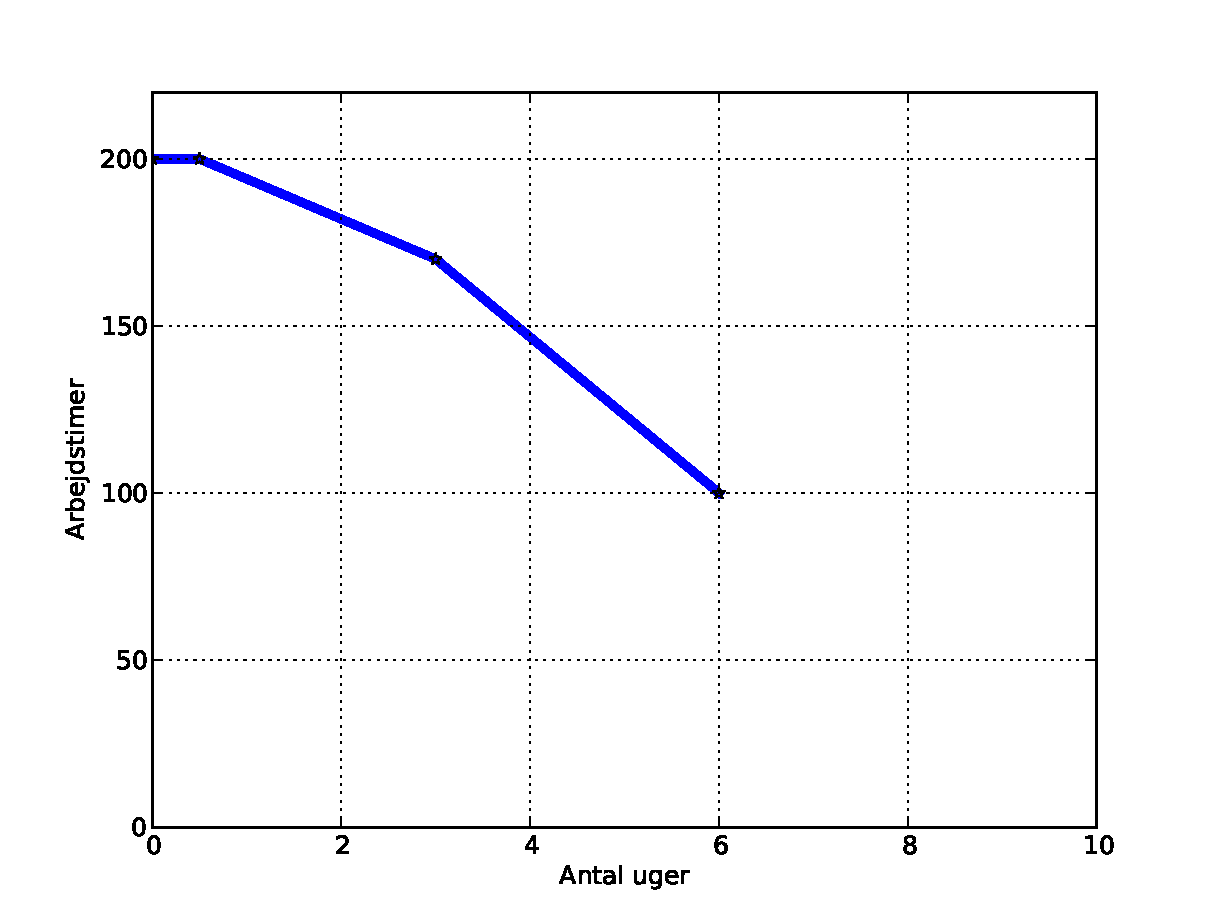
\includegraphics[width=13cm, height=9cm]{burn.pdf}
%\caption{Burndown diagram over projektforløbet}
\label{fig:bd}
\end{figure}
\begin{center}
\textbf{Figur 9:} Burndown diagram over projektforløbet
\end{center}

Vi har som udgangspunkt afsat mellem 8 og 10 uger til det agile projektforløb og bedømt den påkrævede arbejdsindsats til at være 200 timer, hvilket vil sige 100
timer til hver, da vi er to mand i gruppen. Dette overslag er dog yderst usikkert, men vi har aldrig prøvet at arbejde på denne måde før, så det bliver spændende at se, om vores estimationer bliver mere præcise undervejs. Vi har
planlagt at udvikle i sprints af 14 dages varighed, men vi kan udvide dette til 3 uger, hvis et af punkterne i produkt backloggen forekommer mere omfangsrigt.\\
Indehaveren af K. Translation har ofte meget travlt og kan som sagt ikke deltage i hvert nyt sprintmøde. Derfor har vi besluttet at simulere disse møder ved, at vi selv skriver og opdater produkt backloggen og gør det med udgangspunkt i kravspecifikationen. Vi bliver herved in effect vores egen 
proxykunde. Den anden produkt backlog kan ses i tabel 5. Den første produkt backlog kan ses i bilag B.

\begin{center}
	\begin{tabular}{|p{8cm}|l|l|l|}
		\hline
Punkt & Prioritet & Værdi & Timer \\ \hline
Som bruger af KT's hjemmeside bliver man præsenteret for en kalender, hvori man
kan booke en aftale med KT. & 1 & Høj &  50 \\ \hline
Som KT's kunde møder skal man have mulighed for at vedhæfte dokumenter, der skal oversættes, til en aftale. & 2 &
Middel & 6  \\ \hline
KT skal have muligheden for løbende at tilføje kunder til databasen. & 3 & Høj
& 15 \\ \hline
Man skal som kunde modtage en bekræftende email efter at have lavet en aftale
i kalenderen. KT skal ligeledes modtage en email med aftalen. & 4 & Middel & 10  \\ \hline
Som kunde bliver man præsenteret for en lille menu, hvor man skal vælge typen
på arbejdet. & 5 & Lav & 20\\ \hline
Som kunde skal man kunne søge i kalenderen ved hjælp af dato eller klokkeslet.
& 6  & Middel &  25 \\ \hline
Indehaveren af KT vil gerne kunne synkronisere sin eksterne kalender med
hjemmesidens kalender og på den måde overføre sine private aftale. & 7 & Lav &
 35 \\ \hline
\end{tabular}
\end{center}
\begin{center}\textbf{Tabel 5} Anden Produkt Backlog
\end{center}
\vspace{0.5cm}

KT's ønsker står i prioriteret rækkefølge, og vi har yderligere tilføjet en kolonne, hvor vi kan estimere nytteværdien af punktet med Høj, Lav eller
Middel. Sidste kolonne viser vores bedømmelse som udviklere af den påkrævede arbejdsindsats. Ofte vil punkterne i produkt backloggen være formuleret som små brugerhistorier eller endda som deciderede use cases. Dernæst har vi valgt ud, hvilke punkter vi koncentrerer os om i den første sprint. Dette fremgår af tabel 6, som er den anden sprint backlog. Den første kan findes i bilag B. Punkterne bliver yderligere delt op i sprint opgaver, og hver udvikler påtager sig et antal opgaver og kommer igen med en bedømmelse af den påkrævede arbejdsindsats i timer. Sprint backloggen bliver dermed udgangspuktet for systemudviklingen i den efterfølgende sprint. 


\begin{center}
	\begin{tabular}{|l|p{4cm}|l|l|}
		\hline
		Backlog punkt & Sprint opgave & Frivillig & Timer\\ \hline
		\multirow{4}{4cm}{Som bruger af KT's hjemmeside bliver man præsenteret for en kalender, hvori man
		kan booke en aftale med KT.} & Oprette en månedskalender & Omar  & 10 \\
		& Oprette dags dato i kalenderen & Morten & 10 \\
		& Lave templates og CSS-kode & Omar & 6 \\
		& Oprette muligheden for at booke en aftale & Morten
		& 8 \\ 
		& Integrer kalenderen med dags dato & Omar og Morten & 6 \\
		& Test af kalender og dags dato & Morten & 5
		\\ & Integrer kalenderen med login-systemet & Omar & 5 \\
		\hline

	\end{tabular}
\end{center}

\begin{center}
\textbf{Tabel 6} Anden Sprint Backlog
\end{center}

\vspace{0.5cm}

\section{System test}
Vi har desværre ikke testmateriale klart, som vi kan præsentere p.t., så i stedet for vil vi beskrive, hvordan vi vil teste vores kode. (Vi vil have det klart til den endelige eksamensrapport). \\
Da vi til en af gæsteforelæsningerne blev præsenteret for et test-system, der hed Go, som automatiserede testningen af et system, ville vi efterfølgende gerne prøve at teste med Go, men vi må nok erkende, at vi ikke har tid til at lære dette program først og så teste vores projekt. I stedet for vil vi bruge Djangos indbyggede testsystem. Vi opretter en fil ved navn test.py, hvor vi indsætter alle vores testfunktioner, og på baggrund af denne fil, kan Django automatisere test arbejdet. Django vil til testen oprette en test-database, som vi kan indsætte emner i, og vi kan så teste på resultatet af diverse operationer. Vi kan også teste om vores viewfunktioner viser den rigtige hjemmeside eller om de returnerer en fejlkode. Til sidst returneres resultatet af testen. Vi kan altså teste vores kalender ved at bruge testdatabasen til at simulere en række af brugerinput og efterfølgende teste, at vores system opfører sig korrekt.  

\section{Projektarbejdet}
For at runde projektarbejdet af vil vi kort beskrive det foreløbige gruppearbejde og kundesamarbejde. Vi har et utroligt godt samarbejde i vores tomandsgruppe, og vi bidrager begge på de områder, hvor vi hver har vores forcer. Da vi kun er to mand i gruppen, er det meget let at træffe beslutninger og derefter føre dem ud i livet. I en større gruppe skal flere personer tages med på råd, og der kan gå rigtig meget tid med diskussioner, og det er vores erfaring, at de kompromiser, hvor alle får lige meget ret, ikke altid er de bedste. Ulempen ved vores tomandsgruppe er, at vi netop ikke får prøvet at diskutere, argumentere for vores ideer og indgå kompromiser i samme omfang som hos en større gruppe, og at dette nok snarere er normen end undtagelsen i erhvervslivet. Hvis vores gruppe var større, kunne det have været spændende, at udpege en decideret Scrum-master til at lede arbejdet, skære igennem og træffe de endelige beslutninger. Denne rolle kunne evt. varetages af en ny person ved hver ny sprint. \\
Vi har i forhold til sidste rapport, haft endnu et kundemøde med Souzane, hvor vi præsenterede hende for det materiale, som vi har på nuværende tidspunkt. Vi gennemgik kort systemet, og hun prøvede de funktioner, der er implementerede. Hun var tilfreds med det nuværende produkt, og vi fortalte hende, hvad vi manglede, og hvordan vi ville fortsætte arbejdet. \\
Samarbejdet med vores kunde, har også været spændende. Souzane er let at arbejde sammen med, men hun ville ikke bruge tid på projektet, hvis hun ikke mente, at kalenderen virkelig kunne gøre en forskel i hendes travle hverdag, så hun stiller samtidig store krav til os. Vi har dog gjort hende det klart, at vi ikke kan garantere at nå i mål med hele projektet, men at vi i så fald må fortsætte med udviklingen på egen hånd i sommerferien. Souzane har et stort netværk, og hun kender mange tolke, der har præcis de samme udfordringer som hende selv, og hun har talt så ivrigt om dette behov for en kalender til tolke, at vi ikke vil afvise, at vi vil arbejde videre med det på egen hånd. \\ 


\section{The M.A.D. experience}
Artiklen handler om et konkret projekt, hvor en arbejdsgruppe på Århus Universitet arbejdede sammen med et privat shippingfirma, som forbliver anonymt. Projektet var udviklingen af en prototype til et globalt customer-service system, og deadlinen var meget stram. De kalder selv processen for hurtig evolutionær prototyping, idet deadlines var stramme og protoypen blev udviklet evolutionært. Undervejs kommer de med mange spændende bud på nytænkning til systemudvikling, og man får på fornemmelsen, at de mener, at de nytænker processen på mange områder. Der kommer bl.a. disse formuleringer undervejs: analyse er andet og mere end at finde verber og navneord, design er mere end at udfylde detaljerne i OO analyse modellen og implementation er andet og mere end at oversætte modellen til kode. Disse slogans blev til på baggrund af deres tilgang til projektet. For det første havde de en etnograf med i projektet, der kunne analysere den sociale organisering af arbejdet i shipppingfirmaet, og præsentere en konkret forståelse af arbejdet i modsætning til idealiserende opfattelser. For det andet blev der afholdt workshops rundt omkring i verden i shippingfirmaets afdelinger, for at få et nøjagtigt billede af arbejdsgangene i firmaet og for at inddrage så mange forskellige folk som muligt. Herved kunne projektgruppen udarbejde designet og protypen i samspil med de potentielle end-users; de kalder det for "coorporative design" eller "participatory design", og vi har før læst  om lignende inddragelse af slut-brugere i prototype-design i artiklen fra Ehn og Kyng "Mocking it up". Det er særdeles vigtig for at kunne bygge bro mellem aktuelle arbejdsgange og fremtidig praksis. For det tredie kommer artiklen ind på objekt-orientering og forholdet mellem modellen, designet og det at formulere en model på baggrund af koncepter, der nedstammer fra praksis.   \\
Artiklen beskriver også, hvordan projektet blev fulgt op af adskillige reviews undervejs; både med firmaets konsulenter og business repræsentanter, men også med ledelsen i firmaet. \\
Men det overordnede punkt i artiklen er den iterative tilgang til udviklingen af prototypen, hvor man nærmest gror en protype. Ikke sekventielt som i et waterfall projektforløb, men iterativt som i agil projektudvikling, som vi også har læst adskillige artikler om bl.a. "Scrum"-artiklen. Det betyder, at de forskellige designfaser kunne foregå samtidig i de forskellige iterationer, så analyse, design, implementation, brugertest kunne optræde side om side. \\
Vi har i de foregående artikler læst om, hvordan mange forskellige folk har prøvet at finde systemudviklingens "silver bullet", vise sten eller hvad man nu skal kalde det. "No silver bullet", " A rational design process: How and why to fake it" og "Designing for usability: key principles and what designers think" handlede alle om  systemudvikling, og artiklernes forfattere opstillede regler, krav, principper for at nå det optimale systemsudviklingsforløb. \\


\section{Programming as theory building}



\pagebreak

\section{Literaturfortegnelse}
\begin{thebibliography}{9}
	\bibitem{oose}
		Bernd Bruegge og Allen H. Dutoit,
		\emph{Object-Oriented Software Engineering Using UML, Patterns
		and Java},
		Pearson Education Limited, Edinburgh,
		Third Edition,
		2014.
	\bibitem{scrum}
		Jeff Sutherland,
		\emph{Jeff Sutherland's Scrum Handbook},
		Scrum Training Institute, Massachusetts,
		Årstal: ?.


\end{thebibliography}

\newpage

\section{Bilag}

\subsection{Bilag A: Mock-ups af kalenderen}

\begin{figure}[!ht]
\begin{center}
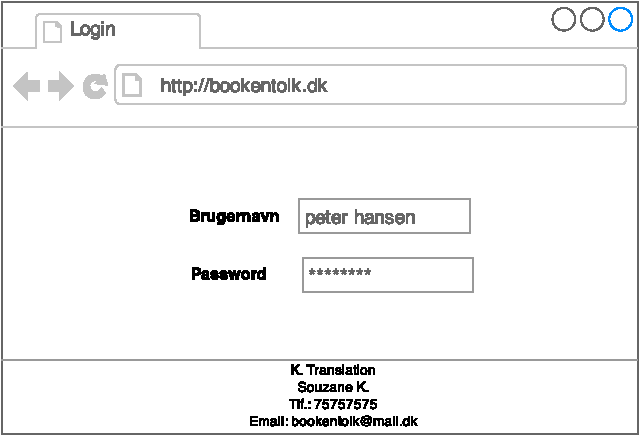
\includegraphics{mock1.pdf}
\caption{Mock-up tegning 1.}
\end{center}
\end{figure}


\newpage

\begin{figure}[!ht]
\begin{center}
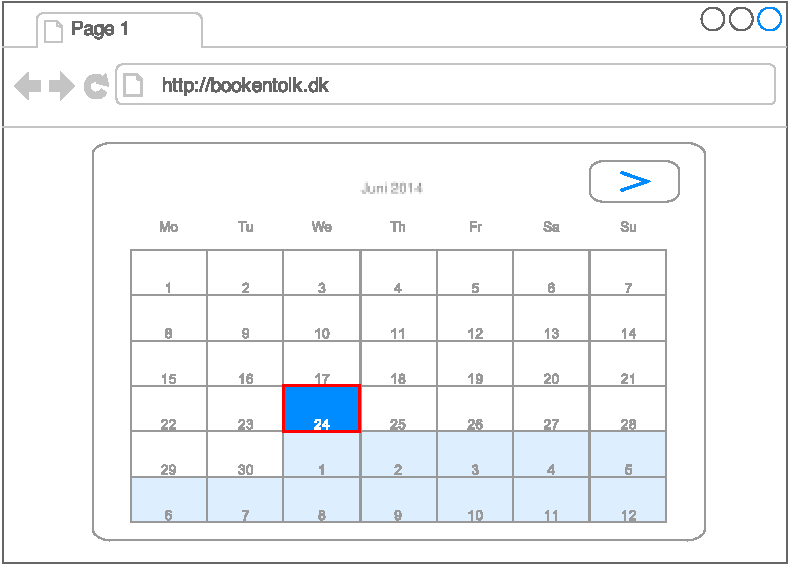
\includegraphics{mock2.pdf}
\caption{Mock-up tegning 2.}
\end{center}
\end{figure}


\newpage

\begin{figure}[!ht]
\begin{center}
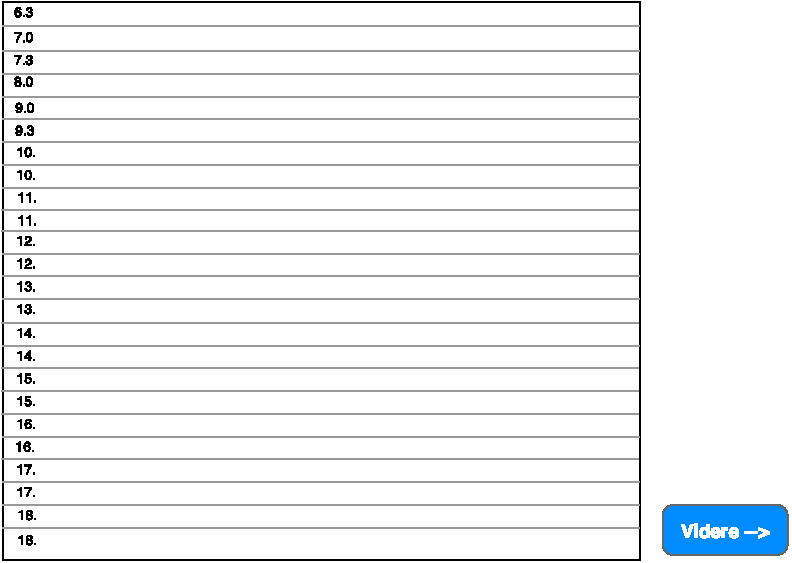
\includegraphics{mock3.pdf}
\caption{Mock-up tegning 3.}
\end{center}
\end{figure}


\newpage

\begin{figure}[!ht]
\begin{center}
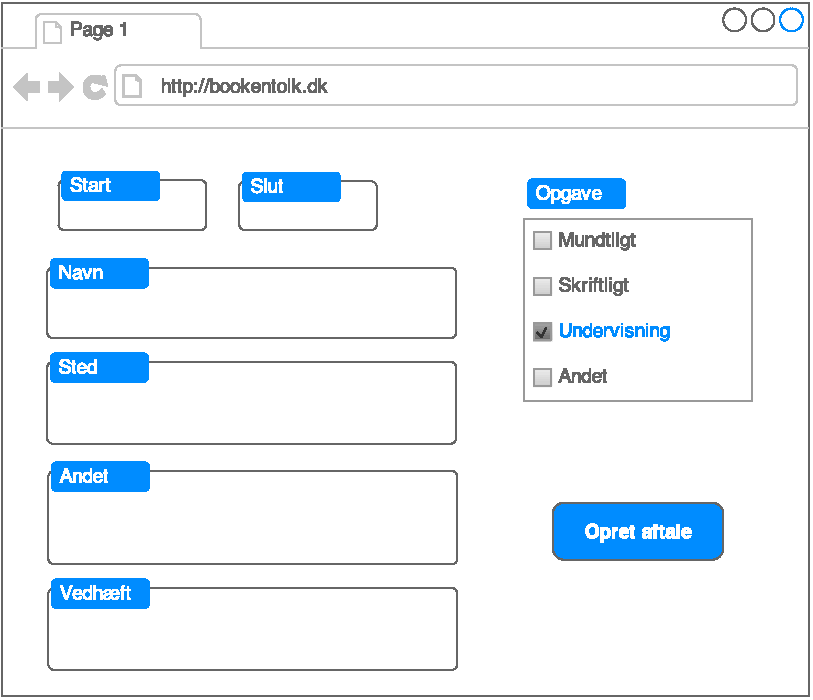
\includegraphics{mock4.pdf}
\caption{Mock-up tegning 4.}
\end{center}
\end{figure}


\newpage

\begin{figure}[!ht]
\begin{center}
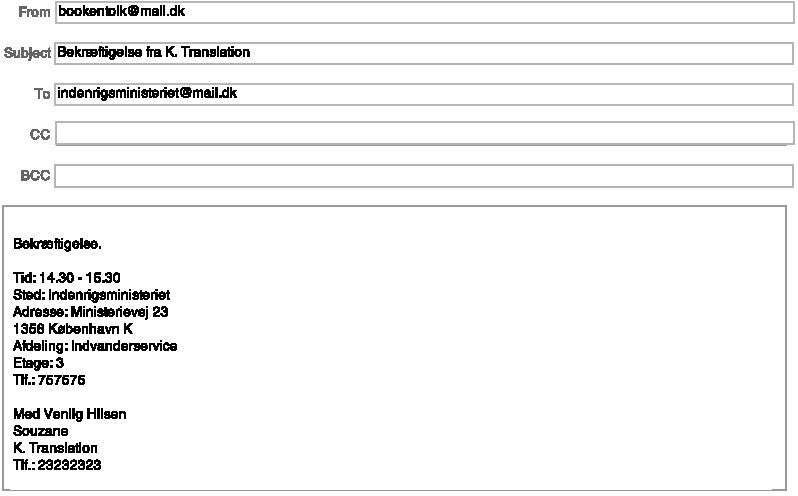
\includegraphics{mock5.pdf}
\caption{Mock-up tegning 5.}
\end{center}
\end{figure}

\newpage

\subsection{Bilag B: Første product- og sprint backlog}

\begin{center}
	\begin{tabular}{|p{8cm}|l|l|l|}
		\hline
Punkt & Prioritet & Værdi & Timer \\ \hline
Som bruger af KT's hjemmeside bliver man præsenteret for en kalender, hvori man
kan booke en aftale med KT. & 1 & Høj &  50 \\ \hline
Som KT's kunde møder man et login interface, når man navigerer til hjemmesiden. & 2 &
Høj & 15  \\ \hline
KT skal have muligheden for løbende at tilføje kunder til databasen. & 3 & Høj
& 15 \\ \hline
Man skal som kunde modtage en bekræftende email efter at have lavet en aftale
i kalenderen. KT skal ligeledes modtage en email med aftalen. & 4 & Middel & 10  \\ \hline
Som kunde bliver man præsenteret for en lille menu, hvor man skal vælge typen
på arbejdet. & 5 & Lav & 20\\ \hline
Som kunde skal man kunne søge i kalenderen ved hjælp af dato eller klokkeslet.
& 6  & Middel &  25 \\ \hline
Indehaveren af KT vil gerne kunne synkronisere sin eksterne kalender med
hjemmesidens kalender og på den måde overføre sine private aftale. & 7 & Lav &
 35 \\ \hline
KT ønsker en hjemmeside med kontaktinformation, billeder og et enkelt design.
& 8 & Middel & 12 \\ \hline
\end{tabular}
\end{center}
\begin{center}\textbf{Første Produkt Backlog}
\end{center}
\vspace{0.5cm}



\begin{center}
	\begin{tabular}{|l|p{4cm}|l|l|}
		\hline
		Backlog punkt & Sprint opgave & Frivillig & Timer\\ \hline
		\multirow{4}{4cm}{Som KT's kunde møder man et login interface,
		når man navigerer til hjemmesiden.} & Oprette en Django
		applikation & Omar  & 2 \\
		& Skriv login interfacet & Morten & 6 \\
		& Test login interfacet & Omar & 3 \\
		& Integrer interfacet med resten af hjemmesiden & Morten og Omar
		& 4 \\ \hline
		\multirow{3}{4cm}{KT ønsker en hjemmeside med
		kontaktinformation, billeder og et enkelt design.} &
		Skrive basisskabelonen til Django & Morten & 5 \\
		& Udvid basisskabelonen med Djangos ``extend''-skabeloner & Morten & 5
		\\ & Test hjemmesiden i flere forskellige browsere & Omar & 2 \\
		\hline

	\end{tabular}
\end{center}

\begin{center}
\textbf{Første Sprint Backlog}
\end{center}

\vspace{0.5cm}

\newpage



\subsection{Bilag C: Referater af kundemøder}

Kundereferat af 1. møde med K.Translation 

Det indledende møde fandt sted på kundens kontor på Østerbro. Kunden havde ved andre sammenhænge givet udtryk for frustrationer og ærgrelser over tabt arbejdsfortjeneste og usammenhængende tider og booking heraf. I denne forbindelse gjorde jeg kunden bekendt med vores  kommende projekt og tilbød vores assistance og stå til rådighed med denne udfordring. 

Det første møde var således kundes og vores ideface og brainstorm, hvor kunden bare frit skulle forklare hvordan disse frustrationer og udfordringer konkret former sig. Det var tydeligt for os som it-konsulenter, at kunden havde et it-behov og ved manglende kompetence var det oplagt at vi skulle hjælpe til og ligge en strategi for hvordan vi på bedst mulig vis kunne gennemføre et succesfuldt projekt. De første spørgsmål som indgik I mødet var således. Hvad er dine udfordringer og hvordan kommer de til udtryk? Hun forklarede at hendes udfordringer var at huske alle de aftaler der var indgået og at kunne bevare overblik over hvem og hvornår der var aftalt tidspunkt for hendes tolkeservicejobs. Derfor ville en mulig it-løsning aflaste de aftener med papir og alle de manuelle indtastninger hun foretog gang på gang.  Hvad tror du kan afhjælpe dine udfordringer.? It-system hvor det hele skulle køre igennem, var hvad hun anså som en problemløser for denne arbejdsmæssige udfordring. For også at kunne gøre det nemmere for hendes samarbejdspartner. Hvor mange samarbejdspartner sammen arbejder du med? Hertil svarede hun at hun havde advokater, politi og retssystemet og somme tide andre ínstitutioner hvor hendes opgave var at oversætte fra arabisk. Hvordan ønsker du systemet? Systemet skal være simpelt og nemt og let tilgængeligt for hende og hendes samarbejdspartnere. 

Vi kom frem til følgende punkter som vi ville arbejde videre på og som var I overensstemmelse med hvilke muligheder og hvilket kompetencer vi kunne tilbyde med dette projekt.  

Efterfølgende blev vi enige om at en konkretisering af hvilke parter som skulle have adgang til systemet og ikke mindst hvordan systemet skulle arbejde var noget vi aftalte vi skulle have på plads til næste møde. Konklusionen og det sidste KT ønskede var at booking systemet skulle være enkelt og ikke for kompliceret. 

\newpage

Referat af andet kundemøde.\\

Deltagere: Omar Khalidan, Souzanne Khalidan, Morten Trolle
Sted: Biocenter. Fredag den 9. maj 2014. Klokken 13 - 14.30.\\

Andet kundemøde startede med, at Souzanne gennemgik hvilke opgavetyper, hun som tolk oftest kommer ud for. Til det formål præsenterede hun os for en række mails og faxbeskeder, hvor hendes samarbejdspartnere havde booket hende til en opgave. I forhold til sidste kundemøde blev kundegrundlaget yderligere udspecificeret, idet hun detaljeret fortalte hvilke samarbejdspartnere, der bruger hende; hvor mange, der bruger hende; på hvilke tidspunkter, de bruger hende. I forhold til det første kundemøde, blev vi måske lidt overraskede over antallet af samarbejdspartnere, som hun anslog til omkring 100. Det blev også præciseret, at det ikke er den samme person hos hver partner, der booker Souzanne, men at der i politiet f.x. godt kan være flere forskellige, der booker hende. \\
I den forbindelse snakkede vi også om brugeroprettelse, og om Souzanne selv skal lægge sine kunder ind i systemet, eller om kunderne opretter sig selv. Vi blev enige om, at Souzanne oprettter de brugere, der er til systemet, da dette vil være det letteste for hendes kunder. Hun vil så præsentere dem for et brugernavn og password, så de efterfølgende kan logge på kalenderen. \\
Vi diskuterede også flere problemstillinger ved selve kalenderen. Souzanne vil gerne have, at brugerne i kalenderen kan se, om hun er optaget, og hvis hun er optaget, om det er fordi, hun slet ikke er til at træffe (f.x. ved ferie), eller om kunderne kan træffe hende telefonisk. Vi snakkede om at løse problemet med forskellige farvekoder for de forskellige aftaletyper, så booket kunne være grøn, ledig kunne være rød osv. \\
Når kunderne booker en tid, skal de også oplyse flere ting, såsom sted, adresse, afdeling, etage, forventet tid, opgavetype (mundtligt, skriftligt, telefonisk). 
Souzanne havde også i forhold til første kundemøde tænkt over, om hendes faktureringssystem på en eller anden måde kunne spille sammen med kalenderen og specielt alle aftalerne i kalenderen. Da hun arbejder meget og derfor har meget travlt, kan hun sagtens glemme at sende en faktura for udført arbejde. Hun ville gerne have denne proces automatiseret på en eller anden måde, og vi sagde, at vi ville undersøge dette uden dog at love hende noget. Evt. kan det være, at vi i sommerferien arbejder videre på systemet og får noget sådant implementeret. \\
Vi kom også ind på spørgsmålet om, hvor det endelige system skal placeres. Det vil være for dyr en løsning for Souzanne og K. Translation at købe en helt ny server til at hoste systemet på, så vi blev enige om, at Omar og jeg finder et webhotel eller en anden udbyder af serverplads. På den måde får Souzanne også så lidt med systemets daglige drift at gøre, og det er en stor prioritet for hende. Vi spurgte også ind til en ønsket hjemmesideadresse, og kom frem til noget i stil med (hvis den er ledig): bookentolk.dk.  
Til sidst snakkede vi også om præsentationen af hjemmesiden. Som det også fremgik på første kundemøde, skal det være så let for kunden som muligt at booke en tid. Derudover vil Souzanne gerne have hjemmesiden holdt i lyse pastelfarver evt. blandet med sort.

\newpage

Referat af tredie kundemøde.\\

Deltagere: Omar Khalidan, Souzanne Khalidan, Morten Trolle
Sted: Diku. Fredag den 30. maj 2014. Klokken 12 - 13.

Vi mødtes med Souzane for tredie gang for at gøre status og lave et kort review af projektet. Vi præsenterede hende for det arbejde, som vi havde lavet siden sidste møde, og hun kunne nu se flere af funktionere i brug. Hun prøvede også selv de funktioner, det var muligt på daværende tidspunkt. Vi forklarede hende så, hvordan vi havde planlagt at fortsætte projektet, og hvilke dele vi stadig manglede at implementere. \\
Souzane var ganske tilfreds med projekt og kalenderen, og vi diskuterede, hvor godt vi havde ramt hendes forventninger, og hvor projektet afviger fra kravspecifikationen. 

\end{document}











